\chapter{MEASUREMENT}\label{chap:3}

\section*{INTRODUCTION}
This module presents a discussion on measurement that includes key concepts like definition
of measurement, development of measurement from primitive to present times, uses and
importance of measurement, systems of measurement, types of measurements such as linear
measures, liquid measures (capacity/volume), and mass or weight. Conversion factors from one unit
to another either within a system or from one system to another are also discussed. Measurement
of time, temperature, and utilities usage (meter reading) are also included. Solving problems using
the formulas on measurement of geometric figures such as perimeter, area, and volume are also
explored.
\section*{OBJECTIVES}
After completing this module, the learner should be able to extend concepts of measurements
to include different types of measures and all the subsets of the set of real numbers to solve
measurement problem. In particular, the learner should be able to:
\begin{enumerate}
\item describe what it means to measure;
\item describe the development of measurement from the primitive to the present international
system of units;
\item convert measurements from one unit to another for each type of measurement including
the English system;
\item estimate or approximate the measures of quantities particularly length, weight/mass,
volume/capacity, time, angle and temperature (use of instruments);
\item use appropriate instruments to measure quantities such as length, weight/mass, volume,
time, angle, and temperature; and
\item solve problems involving formulas in finding perimeter, area, and volume.
\end{enumerate}
\section*{DISCUSSION}
\subsection*{Motivation}
Answer the following questions.
\begin{enumerate}
\item Which of the following line segments is the longest? Which is the shortest?

\begin{tikzpicture}
\draw (0,0) -- (2,0);
\node [below] at (0,0) {A};
\node [below] at (2,0) {B};
\begin{scope}[xshift=3cm]
\draw (0,0) -- (3,0);
\node [below] at (0,0) {C};
\node [below] at (3,0) {D};
  \begin{scope}[xshift=4cm]
	\draw (0,0) -- (1.5,0);
	\node [below] at (0,0) {E};
	\node [below] at (1.5,0) {F};
	\end{scope}
\end{scope}
\end{tikzpicture}
\item Which of the given figures occupy more space than the others?

\begin{tikzpicture}
\draw (0,0) rectangle (3,2);
\begin{scope}[xshift=4cm]
\draw (0,0) -- (1.5,1) -- (3,0) -- cycle;
	\begin{scope}[xshift=4cm,yshift=-1cm]
	\draw (0,0) rectangle (3,3);
	\end{scope}
\end{scope}
\end{tikzpicture}
\item Which of the given containers have more liquid than the others?

\begin{tikzpicture}
\draw (0,0) ellipse (2 and 0.5);
\draw (-2,0) -- (-2,-2);
\draw (-2,-2) arc (180:360:2 and 0.5);
\draw (2,-2) -- (2,0);
	\begin{scope}[xshift=4cm]
	\draw (0,0) ellipse (1.5 and 0.5);
	\draw (-1.5,0) -- (-1.5,-3);
	\draw (-1.5,-3) arc (180:360:1.5 and 0.5);
	\draw (1.5,-3) -- (1.5,0);	
		\begin{scope}[xshift=3.5cm]
		\draw (0,0) ellipse (1.25 and 0.5);
		\draw (-1.25,0) -- (-1.25,-3.5);
		\draw (-1.25,-3.5) arc (180:360:1.25 and 0.5);
		\draw (1.25,-3.5) -- (1.25,0);	
		\end{scope}
	\end{scope}
\end{tikzpicture}
\end{enumerate}
How do you answer these questions? To be able to answer these questions you need to
compare one figure with the other figures. Then you compare also the quantities or the
properties of these figures. The process of comparing one quantity with another quantity is
known as \Bold{measurement}.

\begin{definition}[Measurement]
\Bold{Measurement} is a quantitative description of a fundamental property or physical
phenomenon. When measuring, comparison of an unknown quantity with a certain
standard called \Bold{unit of measurement} is being done.

The science of measurement is called \Bold{metrology}. The English word \Ital{measurement}
originates from the Latin \Ital{m\-ens\-ura} and the verb \Ital{metiri} through the Middle French \Ital{mesure}.
\end{definition}

\subsection*{Historical Background}
Standard units of measurement were already used in ancient times. It evolved over
the course of human history to help prevent problems on fraud in commerce. Laws
regulating measurement were developed so that communities would have certain common
benchmarks. Generally, units of measurement are essentially arbitrary; groups of people
make them up as the need arises, and then agree on certain standards when they use them.

Ancient people used human body parts (arms, hands, feet) to measure length. The
width of a finger was called a \Bold{finger} or \Bold{digit}. Another unit of measure used was the \Bold{palm}
which was the width of a person’s four fingers excluding the thumb. A \Bold{span} was the width of
three palms. The \Bold{cubit} was described as the distance from a man’s elbow to the tip of his
middle finger. Genesis 6: 15 of the Bible stated that Noah’s ark was 300 cubits long, 50
cubits wide and 30 cubits high. One cubit was equivalent to seven palms. The width of a
person’s thumb was called \Bold{uncia}. One foot was equivalent to twelve uncias. The \Bold{yard}, based
on the distance from the tip of a person’s nose to the tip of his middle finger, was
equivalent to three feet. Ancient people also used the \Bold{king’s foot} as the standard unit of
measure for buying, selling, and trading as long as the king ruled. A \Bold{fathom} was the distance
from one outstretched hand to the other, and was equivalent to four cubits.

Eventually, size variations of the different body parts created measurement
problems. Different measurements would be given for the same length using the same unit.
To eliminate such confusion, international conventions were conducted to set standard
units of measure.

\subsection*{International Treaties (Optional)}
Units of measurement are generally defined on a scientific basis as overseen by
governmental or supra-governmental agencies, and established in international treaties.
\Bold{The General Conference on Weights and Measures (CGPM)} which was established in 1875
by the Treaty of the meter oversees the \Bold{International System of Units (SI)} and has custody
of the \Bold{International Prototype Kilogram}. The \Bold{meter} was redefined in 1983 by the CGPM as
the \Ital{distance traveled by light in free space in 1/299,792,458 of a second} while in 1960 the
\Bold{international yard} was defined by the governments of the United States, United Kingdom,
Australia and South Africa as being \Ital{exactly} 0.9144 meters.

In the United States, the \Bold{National Institute of Standards and Technology (NIST)}, a
division of the United States Department of Commerce, regulates commercial
measurements. In the United Kingdom, the one doing this job is the National Physical
Laboratory (NPL). In Australia it is done by the Commonwealth Scientific and Industrial
Research Organization. In South Africa the one doing this is the Council for Scientific and
Industrial Research, while in India the National Physical Laboratory of India does this job.

\subsection*{Units and Systems of Measurement}
\begin{figure}[h]
\centering
\includegraphics[width=2in]{milkbottle}
\caption{A baby bottle that measures in all three measurement systems, Imperial (U.K.), U.S. customary, and
metric.}
\label{fig3:1}
\end{figure}

\begin{figure}[h]
\centering
\includegraphics[width=2in]{measuringdev}
\caption{Four measuring devices having metric calibrations}
\label{fig3:2}
\end{figure}

\subsection*{Linear Measures}
To measure lengths or distances, linear measures are used. An inch is the smallest
and commonly used linear unit in the English system. In this system, other units such as foot,
yard, and mile are used for longer distances. In the metric system the basic unit of length is
the meter. The meter is the basis of other units of measurements such as the decimeter,
centimeter and millimeter. To measure longer distances, the decameter, hectometer and
kilometer are used.

\subsection*{Liquid Measures}
To measure volume (the space occupied by a liquid substance), liquid measures are
used. The basic liquid measures in the English system are the fluid ounce and the gallon. In
the metric system, liter is the basic unit.

\subsection*{The Dry Measure}
The dry measure is used for measuring grains, fruits, vegetables, and the like. The
English system uses pints and quarts as the units for dry measures and for liquid measures.
The metric system also uses the same unit for measuring both liquid and dry substances.

\subsection*{Mass and Weight}
Mass was used by Newton to mean the quantity of matter, and it mass manifests
itself gravitationally and inertially. The earth’s gravitational pull on an object depends on the
object’s mass. The greater the mass of the object, the stronger the earth’s gravitational pull
on it. Mass depends only on the number and kinds of atoms that compose an object. It
does not depend on location. The amount of material in an object remains the same
whether it is located on Earth, on the moon or in outer space. Mass is also a measure of the
inertia of an object. The greater the mass of an object, the greater is its inertia and the more
force is needed to change its state of motion. Mass is measured in ounces (oz), pounds (lb)
and tons in the English system, while it is measured in grams (g) and kilograma (kg) in the
metric system.

Weight is described as a force. Weight is the earth’s gravitational force acting on an
object. It is measured in Newtons (N) like any other force. It depends on the object’s
location and how strongly the object is attracted by the earth’s gravity. The weight of an
object in a place without gravity would be zero.

Mass and weight are different from each other. Mass is the amount of matter in an
object while weight is how that matter is strongly attracted by the force of gravity.
Moreover, mass does not change and does not depend on the location, while weight varies
with location. However, they are proportional to each other in a certain place. Greater
masses have greater weights while smaller masses have smaller weights. This is the reason
why in some cases, mass and weight are used interchangeably. In free fall, (no net
gravitational forces) objects lack weight but retain their mass.

One device for measuring weight or mass is called a weighing \Ital{scale} or, often, simply
a scale. A spring scale measures force but not mass, and a balance compares weight. Both
require a gravitational field to operate. Some of the most accurate instruments for
measuring weight or mass are based on load cells with a digital read-out, but require a
gravitational field to function and would not work in free fall.

\section*{English Customary Weights and Measures}
\subsection*{Linear Measure or Distance}
Short distance units in all traditional measuring systems are based on the dimensions
of the human body. The inch represents the width of a thumb; in many languages, the word
for "inch" is also the word for "thumb." The foot (12 inches) was originally the length of a
human foot, but has evolved to be longer than most people's feet. The yard (3 feet) was
used in England as the name of a 3-foot measuring stick, but it is also understood to be the
distance from the tip of the nose to the end of the middle finger of the outstretched hand. If
you stretch your arms out to the sides as far as possible, your total "arm span," from one
fingertip to the other, is a fathom (6 feet).

Based on history, many other "natural units" of the same kind were used such as the
following: the digit (the width of a finger, 0.75 inch), the nail (length of the last two joints of
the middle finger, 3 digits or 2.25 inches), the palm (width of the palm, 3 inches), the hand
(4 inches), the shaftment (width of the hand and outstretched thumb, 2 palms or 6 inches),
the span (width of the outstretched hand, from the tip of the thumb to the tip of the little
finger, 3 palms or 9 inches), and the cubit (length of the forearm, 18 inches).

\subsection*{Mass/Weight}
The basic traditional unit of weight, the pound, originated as a Roman unit and was
used throughout the Roman Empire. The Roman pound was divided into 12 ounces, but
many European merchants preferred to use a larger pound of 16 ounces, perhaps because a
16-ounce pound is conveniently divided into halves, quarters, or eighths. During the Middle
Ages there were many different pound standards in use, some of 12 ounces and some of 16.
The use of these weight units naturally followed trade routes, since merchants trading along
a certain route had to be familiar with the units used at both ends of the trip.

The oldest English weight system has been used since the time of the Saxon kings. It
is based on the 12-ounce troy pound, which provided the basis on which coins were minted
and gold and silver were weighed. Since Roman coins were still in circulation in Saxon times,
the troy system was designed to model the Roman system directly. The troy pound weighs
5760 grains, and the ounces weigh 480 grains. Twenty pennies weighed an ounce, and
therefore a pennyweight is $480/20 = 24$ grains. The troy system continued to be used by
jewelers and also by druggists until the nineteenth century. Even today gold and silver prices
are quoted by the troy ounce in financial markets everywhere.

Since the troy pound was smaller than the commercial pound units used in most of
Europe, medieval English merchants often used a larger pound called the "mercantile"
pound (\LATIN{libra mercatoria}). This unit contained 15 troy ounces, so it weighed 7200 grains. This
unit seemed about the right size to merchants, but its division into 15 parts, rather than 12
or 16, was very inconvenient. Around 1300 the mercantile pound was replaced in English
commerce by the 16-ounce avoirdupois pound. This is the pound unit still in common use in
the U.S. and Britain. Modeled on a common Italian pound unit of the late thirteenth century,
the avoirdupois pound weighs exactly 7000 grains. The avoirdupois ounce, 1/16 pound, is
divided further into 16 drams.

Unfortunately, the two English ounce units don't agree: the avoirdupois ounce is
$7000/16 = 437.5$ grains while the troy ounce is $5760/12 = 480$ grains. Conversion between
troy and avoirdupois units is so awkward, no one wanted to do it. The troy system quickly
became highly specialized, used only for precious metals and for pharmaceuticals, while the
avoirdupois pound was used for everything else.

\subsection*{Liquid Measure or Capacity or Volume}
The names of the traditional volume units are the names of standard containers.
Until the eighteenth century, it was very difficult to measure the capacity of a container
accurately in cubic units, so the standard containers were defined by specifying the weight
of a particular substance, such as wheat or beer, that they could carry. Thus the gallon, the
basic English unit of volume, was originally the volume of eight pounds of wheat. This
custom led to a multiplicity of units, as different commodities were carried in containers of
slightly different sizes.

Gallons are always divided into 4 quarts, which are further divided into 2 pints each.
For larger volumes of dry commodities, there are 2 gallons in a peck and 4 pecks in a bushel.
Larger volumes of liquids were carried in barrels, hogsheads, or other containers whose size
in gallons tended to vary with the commodity, with wine units being different from beer and
ale units or units for other liquids.

For liquids Americans preferred to use the traditional British wine gallon, which
Parliament defined to equal exactly 231 cubic inches in 1707. As a result, the U.S. volume
system includes both "dry" and "liquid" units, with the dry units being about 1/6 larger than
the corresponding liquid units.

On both sides of the Atlantic, smaller volumes of liquid are traditionally measured in
fluid ounces, which are at least roughly equal to the volume of one ounce of water. To
accomplish this in the different systems, the smaller U.S. pint is divided into 16 fluid ounces,
and the larger British pint is divided into 20 fluid ounces.

On both sides of the Atlantic, smaller volumes of liquid are traditionally measured in
fluid ounces, which are at least roughly equal to the volume of one ounce of water. To
accomplish this in the different systems, the smaller U.S. pint is divided into 16 fluid ounces,
and the larger British pint is divided into 20 fluid ounces.

Because of their many eccentricities, English customary units clearly are more
cumbersome to use than metric units in trade and in science. As metrication proceeds, they
are less and less in use. On the other hand, these traditional units are rich in cultural
significance. We can trace their long histories in their names and relationships.

The units of measure of length, volume and mass /weight in English system are given
in the Table \eqref{chap3tab:1} below. These units are used as conversion factors from one unit of measure to
another.

\begin{table}
\centering
\caption{English System of Measurement}
\begin{tabular}{ll}
\hline
\hline
Linear Measures & Equivalent Unit Measure\\
\hline \hline
12 inches (in) & 1 foot (ft)\\
3 feet & 1 yard (yd)\\
$5\frac{1}{2}$ yards & 1 rod\\
40 rods & 1 furlong\\
8 furlongs & 1 statute mile\\
3 miles & 1 league\\
3 inches & 1 palm\\
4 inches & 1 hand\\
6 inches & 1 span\\
18 inches & 1 cubit\\
21.8 inches & 1 Bible cubit\\
$2\frac{1}{2}$ feet &1 military pace\\
5, 280 feet or 1,760 yards & 1 mile\\
\hline
\hline
Liquid Measures & Equivalent Unit Measures\\
\hline \hline
2 cups (c) & 1 pint\\
2 pints (pt) & 1 quart\\
4 quarts (qt) & 1 gallon (gal)\\
3 teaspoons (tsp) & 1 tablespoon (tbs)\\
8 fluid ounces (fl. oz) & 1 cup\\
16 fluid ounces & 1 pint\\
\hline
\hline
Dry Measures & Equivalent Unit Measures\\
\hline \hline
\multicolumn{2}{c}{(Used for measuring grains, fruits, vegetables, etc.)}\\
2 pints & 1 quart\\
8 quarts & 1 peck(pk)\\
4 pecks & 1 bushel (bu)\\
4 quarts & 1 gallon\\
\hline
\hline
Measures of Mass /Weight & Equivalent Unit Measures\\
\hline \hline
Avoirdupois Weight & \\
27 11/32 grams & 1 dram\\
16 drams &1 ounce (oz)\\
28.3495 grams &1 ounce\\
16 ounces &1 pound (lb)\\
454 grams &1 pound\\
28 pounds &1 quarter (qtr)\\
4 quarters &1 cwt\\
2,000 pounds &1 short ton\\
2,240 pounds &1 long ton\\
\hline
\hline
Troy Weight & Equivalent Unit Measure\\
\hline \hline
24 grains & 1 pennyweight (pwt)\\
20 pennyweight & 1 ounce\\
12 ounces & 1 pound\\
\multicolumn{2}{c}{(Used for weighing gold, silver and jewels)}\\
\hline
\end{tabular}
\label{chap3tab:1}
\end{table}

\subsection*{The Metric System}
The metric system is a decimal system of measurement based on its units for length,
the meter and for mass, the kilogram. It exists in several variations, with different choices of
base units. Since the 1960s, the International System of Units (SI) is the internationally
recognized metric system. Metric units of mass, length, and electricity are widely used
around the world for both everyday and scientific purposes.

The metric system features a single base unit for many physical quantities. Other
quantities are derived from the standard SI units. Multiples and fractions of the units are
expressed as powers of 10 of each unit. Unit conversions are always simple because they
are in the ratio of ten, one hundred, one thousand, etc, so that convenient magnitudes for
measurements are achieved by simply moving the decimal place: 1.234 meters is 1234
millimeters or 0.001234 kilometers. The use of fractions, such as 2/5 of a meter, is not
prohibited, but uncommon. All lengths and distances, for example, are measured in meters,
or thousandths of a meter (millimeters), or thousands of meters (kilometers). There is no
profusion of different units with different conversion factors as in the Imperial system which
uses, for example, inches, feet, yards, fathoms, rods.

The metric system replaces all the traditional units, except the units of time and of
angle measure, with units satisfying three conditions:

\begin{enumerate}
\item One fundamental unit is defined for each quantity. These units are now defined precisely
in the International System of Units.
\item Multiples and fractions of these fundamental units are created by adding prefixes to the
names of the defined units. These prefixes denote powers of ten, so that metric units are
always divided into tens, hundreds, thousands, etc. The original prefixes included milli- for
1/1,000, centi- for 1/100, deci- for 1/10, deka- for 10, hecto- for 100, and kilo- for 1,000.
\item The fundamental units are defined rationally and are related to each other in a rational
fashion.
\end{enumerate}

The metric units were defined in a different way from any traditional units of
measure. The Earth was selected as the “measuring stick”. The meter was defined to be one
ten-millionth of the distance from the Equator to the North Pole. The liter was to be the
volume of one cubic decimeter, and the kilogram was to be the weight of a liter of pure
water.

The metric system was first proposed in 1791. It was adopted by the French
revolutionary assembly in 1795, and the first metric standards (a standard meter bar and
kilogram bar) were adopted in 1799. There was considerable resistance to the system at
first, and its use was not made compulsory in France until 1837. The first countries to
actually require use of the metric system were Belgium, the Netherlands, and Luxembourg,
in 1820.

The units of measure of length, volume and mass/weight in metric system are given in
the Table \eqref{chap3tab:2} below. These units are used as conversion factors from one unit of measure to
another. Dekameter decameter

\begin{table}
\centering
\caption{Metric System}
\begin{tabular}{ll}
\hline \hline
Linear Measures & Equivalent Unit Measure\\
\hline
10 millimeters (mm) & 1 centimeter (cm)\\
10 centimeters & 1 decimeter (dm)\\
10 decimeters & 1 meter (m)\\
100 centimeters & 1 meter\\
1,000 millimeters & 1 meter\\
10 meters &1 decameter (dkm)\\
10 decameters &1 hectometer (hm)\\
100 meters &1 hectometer\\
10 hectometers &1 kilometer (km)\\
1,000 meters &1 kilometer\\
\hline
 & \\
\hline
\hline
Liquid Measures &Equivalent Unit Measures\\
\hline
10 milliliters (ml) &1 centiliter (cl)\\
10 centiliters &1 deciliter (dl)\\
10 deciliters &1 liter (l)\\
100 centiliters &1 liter\\
1,000 milliliters &1 liter\\
10 liters &1 decaliter (dkl)\\
10 decaliters &1 hectoliter (hl)\\
10 hectoliters &1 kiloliter (kl)\\
1 cubic centimeter (cc) &1 milliliter (ml)\\
1,000 cubic centimeters &1,000 milliliters\\
1,000 milliliters &1 liter\\
1,000 liters &1 cubic meter (m$^3$)\\
\hline
& \\
\hline
\hline
Measures of Mass /Weight &Equivalent Unit Measures\\
\hline
10 milligrams &1 centigram (cg)\\
10 centigrams &1 decigram (dg)\\
10 decigrams &1 gram (g)\\
100 centigrams &1 gram\\
1,000 milligrams &1 gram\\
10 grams &1 decagram (dkg)\\
10 decagrams &1 hectogram (hg)\\
100 grams &1 hectogram\\
10 hectograms &1 kilogram (kg)\\
100 kilograms &1 quintal (ql)\\
10 quintals &1 ton (t)\\
\hline
\end{tabular}
\label{chap3tab:2}
\end{table}

\subsection*{International System of Units}
The International System of Units (abbreviated as SI from the French language name
\Ital{Système International d'Unités}) is the modern revision of the metric system. It is the world's
most widely used system of units, both in everyday commerce and in science. The SI was
developed in 1960 from the meter-kilogram-second (MKS) system, rather than the
centimeter-gram-second (CGS) system, which, in turn, had many variants. During its
development, the SI also introduced several newly named units that were previously not a
part of the metric system. The original SI units for the six basic physical quantities were:
\begin{center}
\begin{tabular}{ll}
meter (m) &SI unit of length\\
second (s) &SI unit of time\\
kilogram (kg) &SI unit of mass\\
ampere (A) &SI unit of electric current\\
degree Kelvin (K) &SI unit of thermodynamic temperature\\
candela (cd) & SI unit of luminous intensity\\
\end{tabular}
\end{center}
The mole was subsequently added to this list and the degree Kelvin renamed the kelvin.

There are two types of SI units, base units and derived units. Base units are the
simple measurements for time, length, mass, temperature, amount of substance, electric
current and light intensity. Derived units are constructed from the base units, for example,
the watt, i.e. the unit for power, is defined from the base units as m$^2\cdot$kg$\cdot$s$^{-3}$. Other physical
properties may be measured in compound units, such as material density, measured in
kg/m$^3$.

\subsubsection*{Converting Prefixes}
The SI allows easy multiplication when switching among units having the same base
but different prefixes. To convert from meters to centimeters it is only necessary to multiply
the number of meters by 100, since there are 100 centimeters in a meter. Inversely, to
switch from centimeters to meters one multiplies the number of centimeters by 0.01 or
divide centimeters by 100.

\subsubsection*{Length}
\begin{figure}[!h]
\centering
\includegraphics[width=2in]{ruler}
\caption{A 2-metre carpenter's ruler}
\label{chap3fig:1}
\end{figure}

A ruler or rule is a tool used in, for example, geometry, technical drawing,
engineering, and carpentry, to measure lengths or distances or to draw straight lines.
Strictly speaking, the \Ital{ruler} is the instrument used to \Bold{rule} straight lines and the calibrated
instrument used for determining length is called a \Ital{measure}, however common usage calls
both instruments \Ital{rulers} and the special name \Ital{straightedge} is used for an unmarked rule.
The use of the word \Ital{measure}, in the sense of a measuring instrument, only survives in the
phrase \Ital{tape measure}, an instrument that can be used to measure but cannot be used to
draw straight lines. As can be seen in the photographs on this page, a two-meter carpenter's
rule can be folded down to a length of only 20 centimeters, to easily fit in a pocket, and a
five-meter-long tape measure easily retracts to fit within a small housing.

\subsubsection*{Some Special Names}
We also use some special names for some multiples of some units as in Table \eqref{chap3tab:3}
\begin{table}[!h]
\centering
\caption{SI Special Names}
\begin{tabular}{ll}
\hline \hline
100 kilograms & 1 quintal\\
1000 kilogram & 1 metric tonne\\
10 years & 1 decade\\
100 years & 1 century\\
1000 years & 1 millennium\\
\hline
\end{tabular}
\label{chap3tab:3}
\end{table}

\subsubsection*{Difficulties}
Since accurate measurement is essential in many fields, and since all measurements are
necessarily approximations, a great deal of effort must be taken to make measurements as
accurate as possible. For example, consider the problem of measuring the time it takes an
object to fall a distance of one meter (about 39 in). Using physics, it can be shown that, in
the gravitational field of the Earth, it should take any object about 0.45 second to fall one
meter. However, the following are just some of the sources of error that arise:
\begin{enumerate}
\item This computation used for the acceleration of gravity 9.8 meters per second squared
(32 ft/s$^2$). But this measurement is not exact, but only precise to two significant
digits.
\item The Earth's gravitational field varies slightly depending on height above sea level and
other factors.
\item The computation of 0.45 second involved extracting a square root, a mathematical
operation that required rounding off to some number of significant digits, in this
case two significant digits.
\end{enumerate}
So far, we have only considered scientific sources of error. In actual practice, dropping
an object from a height of a meter stick and using a stopwatch to time its fall, we have other
sources of error:
\begin{enumerate}
\item Most common, is simple carelessness.
\item Determining the exact time at which the object is released and the exact time it hits
the ground. There is also the problem that the measurement of the height and the
measurement of the time both involve some error.
\item Air resistance
\end{enumerate}
Scientific experiments must be carried out with great care to eliminate as much error as
possible, and to keep error estimates realistic.

\subsection*{Metric-English Relationship}
Table \eqref{chap3tab:4} shows the comparison between the Metric and English Systems of
Measurements.
\begin{table}[!h]
\centering
\caption{Metric-English Conversions}
\begin{tabular}{ll}
\hline \hline
Linear Measures &Equivalent Measure\\
\hline
Metric & English\\
1 millimeter & 0.04 inches\\
1 centimeter & 0.39 inches\\
1 decimeter & 3.94 inches\\
1 meter & 39.37 inches\\
1 meter & 3.28 feet\\
1 meter & 1.09 yards\\
1 decameter & 32.81 feet\\
1 hectometer & 328.08 feet\\
1 kilometer & 3,280.80 feet\\
1 kilometer & 0.62 mile\\
25.40 millimeter & 1 inch\\
2.54 centimeters & 1 inch\\
0.03 meter & 1 inch\\
0.30 meter & 1 foot\\
0.91 meter & 1 yard\\
1.61 kilometers & 1 mile\\
\hline
 & \\
\hline \hline
Liquid Measures & Equivalent Measures\\
\hline
Metric &English\\
1 milliliter & 0.03 fluid ounce\\
1 centiliter &0.34 fluid ounce\\
1 deciliter &3.38 fluid ounce\\
1 liter &1.06 liquid quarts\\
1 liter &0.91 dry quart\\
1 decaliter &2.64 gallons\\
1 hectoliter &26.42 gallons\\
1 kiloliter &264.18 gallons\\
0.95 liter &1 liquid quart\\
1.10 liters &1 dry quart\\
3.80 liter &1 gallon\\
\hline
 & \\
\hline \hline
Measures of Mass &Equivalent Measures\\
\hline
Metric &English\\
1 milligram &0.02 grain\\
1 centigram &0.15 grain\\
1 decigram &1.54 grains\\
1 gram &0.04 ounce\\
1 decagram &0.35 ounce\\
1 hectogram &3.53 ounces\\
1 kilogram &2.20 pounds\\
1 metric ton &2,204.62 pounds\\
1 metric ton &1.10 tons\\
28.35 grams &1 ounce\\
0.45 kilogram &1 pound\\
0.91 metric ton &1 ton\\
\hline
\end{tabular}
\label{chap3tab:4}
\end{table}

\subsubsection*{Conversion from One Unit to Another}
The following illustrative examples show how to convert one measure from one unit to
another.
\subsubsubsection{English Units of Measure}
\begin{example}
\item Convert 7 yards to feet. Conversion factor: 1 yd $= 3$ ft

Solution: $7\yd\cdot \dfrac{3\ft}{1\yd}=\boxed{21\ft}$

\item Convert 72 inches to feet. Conversion factor: 1 ft $= 12$ in

Solution: $72\mathrm{in}\cdot\dfrac{1\mathrm{ft}}{12\IN}=\boxed{6\ft}$

\item Convert 14.25 gallons to quarts. Conversion factor: 1 gal $= 4$ qt

Solution: $14.2\gal\cdot\dfrac{4\qt}{1\gal}=\boxed{57\qt}$
\end{example}
\subsubsubsection{Metric Units of Measure}
\begin{example}
\item Convert 8 meters to centimeters. Conversion factor: 1 m $= 100$ cm

Solution: $8\m\cdot \dfrac{100\cm}{1\m}=\boxed{800\cm}$

\item Convert 3 liters to millimeters. Conversion factor: $1 \Li = 1000 \mL$

Solution: $3\Li\cdot\dfrac{1000\mL}{1\Li}=\boxed{3,000\mL}$

\item Convert 250 millimeters to decimeters. Conversion factors: $1 \cm = 10 \mm$, $1\dm = 10
\cm$, hence, $1 \dm = 100 \m$

Solution: $250\mm\cdot\dfrac{1\cm}{10\mm}\cdot\dfrac{1\dm}{10\cm}=\boxed{2.5\dm}$

\item Convert 4,625 centimeters to meters. Conversion factor: $1 \m = 100 \cm$

Solution: $4,625\cm\cdot\dfrac{1\m}{100\cm}=\boxed{46.25\m}$
\end{example}

\subsubsubsection{Metric to English and Vice Versa}
\begin{example}
\item Convert 12 meters to yards. Conversion factor: $1 \m = 1.09 \yd$

Solution: $12\m\cdot\dfrac{1.09\yd}{1\m}=\boxed{13.08\yd}$

\item Convert 10 miles to meters. Conversion factor: $1 \mi = 1.61 \km$, $1 \km = 1000 \m$

Solution: $10\mi\cdot\dfrac{1.61\km}{1\mi}\cdot\dfrac{1000\m}{1\km}=\boxed{16,100\m}$

\item Convert $400 \oz$ to grams. Conversion factor: $1 \oz = 28.35 \g$

Solution: $400\oz\cdot\dfrac{28.35\g}{10\oz}=\boxed{11,340\g}$
\end{example}

\subsection*{Exercises}
\begin{enumerate}[A.]
\item Write the abbreviations of the following units of measure.
	\begin{multicols}{3}
	\begin{enumerate}[1.]
	\item foot
	\item meter
	\item inch
	\item hectometer
	\item millimeter
	\item kilometer
	\item yard
	\item mile
	\item gallon
	\item pint
	\item liter
	\item pound
	\item ounces
	\item grain
	\item millimeter
	\end{enumerate}
	\end{multicols}
\item Write either weight, linear, time, or capacity in each blank to denote the type of measure.
	\begin{multicols}{2}
	\begin{enumerate}[1.]
	\item \answerline{foot}
	\item \answerline{gallon}
	\item \answerline{pint}
	\item \answerline{yard}
	\item \answerline{gram}
	\item \answerline{cup}
	\item \answerline{liter}
	\item \answerline{peck}
	\item \answerline{day}
	\item \answerline{century}
	\end{enumerate}
	\end{multicols}
\item Fill in the blank with the correct number.
	\begin{enumerate}[1.]
	\item \Line $\ft=1\yd$
	\item \Line $\T = 1\yd$
	\item \Line $\dm = 1\m$
	\item \Line $\IN = 1 \yd$
	\item \Line $\ft = 1 \mi$
	\item \Line $\m = 1 \dkm$
	\item \Line $\cm = 1 \dm$
	\item \Line $\dm = 1 \km$
	\end{enumerate}
\item Convert. Use mixed numbers or decimals if necessary.
	\begin{multicols}{2}
	\begin{enumerate}[1.]
	\item $24 \yd = \Line \ft$
	\item $6 \mi = \Line \yd$
	\item 72 in =  ft
	\item 17 ft = \Line in
	\item 7 mi = \Line ft
	\item 1/4 mi = \Line yd
	\item 90 in = \Line yd
	\item 7 ft = \Line yd
	\item 6 mi = \Line in
	\item 14 m = \Line dm
	\item 85 km = \Line dkm
	\item 12 mm = \Line m
	\item 8 m = \Line cm
	\item 1hm = \Line m
	\item 45 m = \Line hm
	\item 83.5 km = \Line hm
	\item 47 dm = \Line m
	\item 145 km = \Line m
	\item 15 ft = \Line  in
	\item 3/4 ft = \Line in
	\item 1.3 mi = \Line ft
	\item 380,160 = \Line mi
	\end{enumerate}
	\end{multicols}
\end{enumerate}

\subsubsection*{Perimeter}
Perimeter is the measure of the total distance around a plane figure. To find the
perimeter of any polygon, the lengths of the sides are added. There are formulas that are
used to make the computation easier and faster.

Table \eqref{chap3tab:5} shows most common shapes and the formula to find the
perimeter of each figure.

\begin{table}[!h]
\centering
\begin{tabularx}{\linewidth}{XXX}
\hline
\hline
Figure & Formula & Description\\
\hline
1. Triangle & $P=a+b+c$ & $a$, $b$, and $c$ are the lengths of
the sides\\
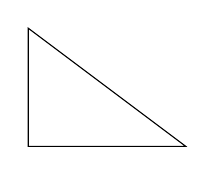
\begin{tikzpicture}
\draw (0,0) -- (2,0) -- (0,1.5) -- cycle;
\end{tikzpicture}
&  & \\
2. Trapezoid & & \\
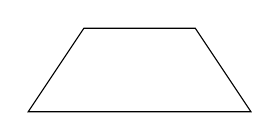
\begin{tikzpicture}[xscale=2]
\draw (0,0) +(135:0.5cm) -- +(45:0.5cm) -- +(-45:1cm) -- +(-135:1cm) -- cycle;
\end{tikzpicture}
 & $P = b_1 + b_2 + s_1 + s_2$ & $b_1$ and $b_2$ are the bases or
parallel sides while $s_1$ and $s_2$
are the nonparallel sides\\
3. Parallelogram & & \\
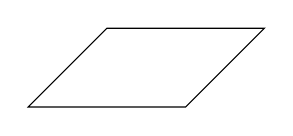
\begin{tikzpicture}
\draw (0,0) -- (2,0) -- (1,-1) -- (-1,-1) -- cycle;
\end{tikzpicture}
 & $P = 2l + 2w$ & $l$ is the length and $w$ is the
width of the parallelogram\\
3. Rectangle & & \\
\tikz \draw (0,0) rectangle (2.5,1.5); & $P = 2L + 2W$ & $L$ is the length and $W$ is the width of the rectangle\\
4. Square & & \\
\tikz \draw (0,0) rectangle (2,2); & $P = 4s$ & $s$ is the length of side of the
square \\
5. Circle & & \\
\tikz \draw (0,0) circle (1cm); & $C=2\pi r=\pi d$ & $r$ is the radius of the circle and $d$ is the diameter; $\pi \approx 3.14$\\
\hline
\end{tabularx}
\caption{Note: A circle is a plane figure whose perimeter is known as the circumference of the circle.}
\label{chap3tab:5}
\end{table}
%\newpage
\subsection*{Exercises}
Find the perimeter of the following.
\begin{multicols}{2}
\begin{enumerate}
\item Square

\begin{tikzpicture}
\draw (0,0) rectangle (2.25,2.25);
\path (0,0) -- (0,2.25) node [midway, left]  {6 cm};
\end{tikzpicture}

\item Rectangle 

\begin{tikzpicture}[scale=1.25]
\draw (0,0) rectangle (2.5,1.25);
\path (0,0) -- (0,1.25) node [midway,left] {3 m};
\path (0,1.25) -- (2.5,1.25) node [midway, above] {6 m};
\end{tikzpicture}

\item Triangle 

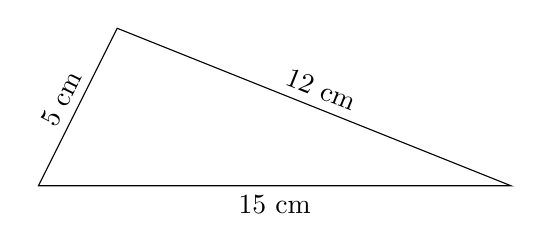
\begin{tikzpicture}[scale=2]
\draw (0,0) -- (3,0) -- (0.5,1) -- cycle;
\path (0,0) -- (0.5,1) node [midway,above,sloped] {5 cm};
\path (0,0) -- (3,0) node [midway, below] {15 cm};
\path (0.5,1) -- (3,0) node [midway, above, sloped] {12 cm};
\end{tikzpicture}

\item Isosceles Trapezoid

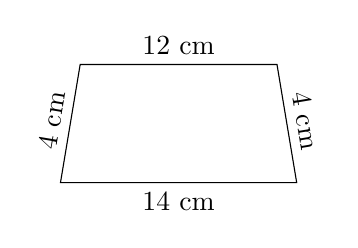
\begin{tikzpicture}
\draw (0,0) -- (3,0) -- (2.75,1.5) -- (0.25,1.5) -- cycle;
\path (0,0) -- (3,0) node [midway,below] {14 cm};
\path (3,0) -- (2.75,1.5) node [midway, above,sloped] {4 cm};
\path (0.25,1.5) -- (2.75,1.5) node [midway,above] {12 cm};
\path (0,0) -- (0.25,1.5) node [midway, above, sloped] {4 cm};
\end{tikzpicture}
\end{enumerate}
\end{multicols}

\subsubsubsection{Area}
The area of a plane figure is the total number of unit regions occupied or contained
in the given plane figure. The unit region is expressed in square units.

\begin{example}
\item The rectangle below has width = 3 units, length = 5 units. There are 15 square
units in the figure. Therefore, the area of the rectangle is 15 square units.

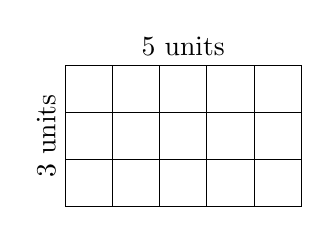
\begin{tikzpicture}[scale=0.6]
\draw (0,0) grid (5,3);
\path (0,3) -- (5,3) node [above, midway] {5 units};
\path (0,0) -- (0,3) node [midway, above, sloped] {3 units};
\end{tikzpicture}
\end{example}

Table \eqref{chap3tab:6} shows most common shapes and the formula to find the area of
each figure.

{\renewcommand{\arraystretch}{1.5}
\begin{table}[!h]
\centering
\caption{Formulas for Areas of Some Common Shapes}
\begin{tabularx}{\linewidth}{XXX}
\hline
\hline
1. Triangle & $A=\dfrac{bh}{2}$ & $A$ is the area, $b$ is the base
and $h$ is the height or
altitude\\
2. Square & $A=s^2$ & $s$ is the length of the side\\
3. Rectangle & $A=lw$ & $l$ is the length and $w$ is the
width\\
4. Parallelogram & $A=bh$ & $b$ is the base and $h$ is the
height or altitude\\
5. Trapezoid & $A=\dfrac{h(b_1+b+2)}{2}$ & $h$ is the altitude and $b_1$ and $b_2$ are the bases\\
6. Circle & $A=\pi r^2$ & $r$ is the radius of the circle; $\pi \approx 3.14$\\
\hline
\end{tabularx}
\label{chap3tab:6}
\end{table}}

\subsection*{Exercises}
Find the area of the following figures:
\begin{enumerate}
\item A square whose side is 9 cm.
\item A rectangle whose width is 2 m and whose length is 5 m.
\item A triangle whose height is 2 cm and whose base is 8 cm.
\item A circle whose diameter is 20 ft.
\item A trapezoid with a height of 8 cm and bases 6 cm and 9 cm.
\end{enumerate}

\subsubsubsection{Volume}
If we want to find how much a box or any container will hold, we need a
measurement of a space. Space involves three dimensions: length, width and height. Any
figure that represents a space is three-dimensional and the measurement of this space is
called volume. The volume is measured in cubic units.

The standard English cubic measures are the cubic inch, cubic foot and the cubic yard.

\begin{center}
1 cubic foot (cu. ft) = 1,728 cubic inches (cu. in)\\
1 cubic yard (cu. yd) = 27 cubic feet (cu. ft)
\end{center}

The standard metric cubic measures are the cubic centimeters and the cubic meters.

Table \eqref{chap3tab:7} shows the formula that are used to solve for the volume of some regular solids.

\begin{table}[!h]
\centering
\caption{Formulas for Volumes of Regular Solids}
\begin{tabularx}{\linewidth}{XXX}
\hline \hline
Figure & Formula & Meaning of Symbols\\
\hline
1. Cube & & \\
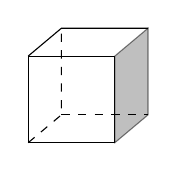
\begin{tikzpicture}[scale=1.1]
\draw (0,0) rectangle (1,1);
\draw [fill=gray,opacity=0.5] (1,0) -- ++(40:0.5cm) -- ++(0,1) -- ++(220:0.5cm) -- cycle;
\draw [dashed] (0,0) -- ++(40:0.5cm) -- ++(0,1);
\draw (0,1) -- ++(40:0.5cm) -- ++(1,0);
\draw [shift=(40:0.5cm),dashed] (0,0) -- (1,0);
\end{tikzpicture}
 & $V=s^3$ & $V=$ volume; $s=$ length of edge\\
2. Rectangular solid & & \\
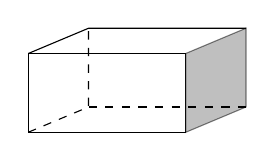
\begin{tikzpicture}[scale=1,xscale=2]
\draw (0,0) rectangle (1,1);
\draw [fill=gray,opacity=0.5] (1,0) -- ++(40:0.5cm) -- ++(0,1) -- ++(220:0.5cm) -- cycle;
\draw [dashed] (0,0) -- ++(40:0.5cm) -- ++(0,1);
\draw (0,1) -- ++(40:0.5cm) -- ++(1,0);
\draw [shift=(40:0.5cm),dashed] (0,0) -- (1,0);
\end{tikzpicture}
 & $V=lwh$ & $V=$ volume; $l=$ length; $w=$ width; $h=$ height\\
3. Square Pyramid & & \\
\begin{tikzpicture}[scale=0.6]
\draw (0,0) -- (2.5,0) -- ++(60:1.5cm);
\draw [dashed] (0,0) -- ++(60:1.5cm) -- ++(2.5,0);
\draw (0,0) -- (1,2.5) -- (2.5,0)
							 (1,2.5) -- ($(2.5,0)+(60:1.5cm)$);
\fill [fill=gray,opacity=0.5] (2.5,0) -- ($(2.5,0)+(60:1.5cm)$) -- (1,2.5) -- cycle;
\draw [dashed] (1,2.5) -- ($(0,0)+(60:1.5cm)$);
\end{tikzpicture}
 & $V=\frac{1}{3}lwh$ & $V=$ volume; $l=$ length; $w=$ width; $h=$ height\\
4. Circular Cylinder & & \\
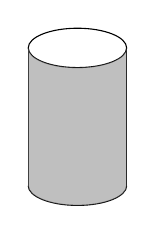
\begin{tikzpicture}[scale=0.5]
		\draw (0,0) ellipse (1.25 and 0.5);
		\draw (-1.25,0) -- (-1.25,-3.5);
		\draw (-1.25,-3.5) arc (180:360:1.25 and 0.5);
		\draw (1.25,-3.5) -- (1.25,0);	
		\fill [gray,opacity=0.5] (-1.25,0) -- (-1.25,-3.5) arc (180:360:1.25 and 0.5) -- (1.25,0) arc (0:180:1.25 and -0.5);
\end{tikzpicture}
 & $V=\pi r^2 h$ & $V=$ volume; $r=$ radius; $h=$ height \\
5. Cone & & \\
\begin{tikzpicture}[scale=1]
\draw [draw=white,left color=insideo,right color=insideo,middle color=insidei] (0,0) ellipse (1 and 0.25);
\shade [left color=insideo,right color=insideo,middle color=insidei] (-1,0) arc (180:360:1 and -0.25) -- (0,2.4) -- cycle;
\draw (-1,0) -- (0,2.4) -- (1,0);
\draw (-1,0) arc (180:360:1 and 0.25) -- (0,2.4) -- cycle;
\draw (-1,0) arc (180:360:1 and -0.25) -- (0,2.4) -- cycle;
\end{tikzpicture}
 & $V=\frac{1}{3}\pi r^2h$ & $V=$ volume; $r=$ radius; $h=$ height \\
6. Sphere & & \\
\begin{tikzpicture}
\draw [left color=white,right color=insideo,middle color=insidei] (0,0) circle (1cm);
\draw (-1,0) arc (180:360:1cm and 0.35cm);
\draw [dashed] (-1,0) arc (180:360:1cm and -0.35cm);
	\begin{scope}[rotate=-90]
	\draw (-1,0) arc (180:360:1cm and 0.35cm);
	\draw [dashed] (-1,0) arc (180:360:1cm and -0.35cm);
	\end{scope}
\end{tikzpicture}
 & $V=\frac{4}{3}\pi r^3$ & $V=$ volume; $r=$ radius; $\pi\approx 3.14$ \\
\hline
\end{tabularx}
\label{chap3tab:7}
\end{table}

\subsubsubsection{Time Measure}
Table \eqref{chap3tab:8} shows the units used to measure time.

\begin{table}[!h]
\centering
\caption{Units of Time}
\begin{tabular}{ll}
\hline \hline
Time Measures & Equivalent Unit Measure\\
\hline
60 seconds & 1 minute\\
60 minutes & 1 hour\\
24 hours & 1 day\\
7 days & 1 week\\
28,29,30 or 31 days & 1 calendar month\\
30 days & 1 month (computing interest)\\
365 days & 1 year\\
366 days & 1 leap year\\
\hline
\end{tabular}
\label{chap3tab:8}
\end{table}

Time reading is done through a clock with 12 numbers on it. The two hands are
called the minute hand and the hour hand. The hour hand indicates the hour reading and
the minute hand represents the minute reading. Some clock has a second hand that reads
the second.

\subsubsubsection{Temperature}
There are two thermometer scales that are commonly used to measure temperature.
These are the Fahrenheit (F) and the Centigrade or Celsius (C). The two scales give
temperature readings in degrees ($^{\circ}$).

\begin{example}
\item $45^{\circ}$ F is read as “forty-five degrees Fahrenheit”
\item $20^{\circ}$ C is read as “twenty degrees Centigrade”
\end{example}

The freezing point of water on the Fahrenheit scale is $32^{\circ}$ F while the boiling point of
water is $212^{\circ}$ F. On the Centigrade scale, the freezing point of water is $0^{\circ}$ C while the boiling
point is $100^{\circ}$. The thermometer is the instrument used to measure temperature.

To change one unit of measure to another unit, we use formulas. The formula used
to change Fahrenheit to Centigrade or Celsius is
\begin{equation}
\mathrm{C}=\frac{5}{9}(\mathrm{F}-32)
\end{equation}
\begin{example}
\item Change $59\degree\F$ to $\degree\C$.

Solution:
\begin{align*}
\C&=\frac{5}{9}(\F-32)\\
&=\frac{5}{9}(27)\\
&=\boxed{15}
\end{align*}
Therefore, $59\degree\F=15\degree\C$.
\end{example}
To change Centigrade to Fahrenheit, we use the formula
\begin{equation}
\F=\frac{9}{5}\C+32
\end{equation}
\begin{example}
\item Change $20\degree\C$ to $\degree\F$

Solution: 
\begin{align*}
\F&=\frac{9}{5}\C+32\\
&=\frac{9}{5}(20)+32\\
&=36+32\\
&=\boxed{68}
\end{align*}
Therefore, $20\degree\C=68\degree\F$.
\end{example}
\subsection*{Exercises}
\begin{enumerate}[A.]
\item Change each of the following to $\degree\C$.
\begin{multicols}{2}
\begin{enumerate}[1.]
\item 72\degree\F.
\item 120\degree\F.
\item 160\degree\F.
\item 84\degree\F.
\item 98\degree\F.
\item 130\degree\F.
\end{enumerate}
\end{multicols}
\item Change each of the following to \degree\F.
\begin{multicols}{2}
\begin{enumerate}[1.]
\item 12\degree\C.
\item 30\degree\C.
\item 35\degree\C.
\item 94\degree\C.
\item 98\degree\C.
\item 75\degree\C.
\end{enumerate}
\end{multicols}
\end{enumerate}

\section*{WORKSHOP ACTIVITIES}
\subsection*{Activity 1: Exercises on Problem Solving Involving Measurements}
\begin{enumerate}
\item If one side of a regular pentagon is 7 cm long, what is its perimeter? (Hint: A regular pentagon has 5 equal sides.)
\item The diameter of a bicycle tire is 50 cm. What is the circumference of the tire?
\item The perimeter of a square is 48 cm. How long is each side?
\item A large pizza has a circumference of 215.2 cm. What is its diameter?
\item The diameter of a wheel is 72 cm. Find its circumference.

Find the area of each of the following by subdividing it into common shapes.
\begin{multicols}{3}
\item 
\begin{tikzpicture}
\draw (0,0) -- (1,0) -- (1,1.5) -- (-0.5,1.5) -- (-0.5,1) -- (0,1) -- cycle;
\path (0,0) -- (1,0) node [below,midway] {2};
\path (0,0) -- (0,1) node [left,midway] {2};
\path (-0.5,1) -- (-0.5,1.5) node [left,midway] {1};
\end{tikzpicture}
\item 
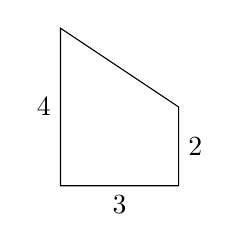
\begin{tikzpicture}[scale=0.5]
\draw (0,0) -- (3,0) -- (3,2) -- (0,4) -- cycle;
\path (0,0) -- (0,4) node [left,midway] {4};
\path (0,0) -- (3,0) node [below,midway] {3};
\path (3,0) -- (3,2) node [right,midway] {2};
\end{tikzpicture}
\item 
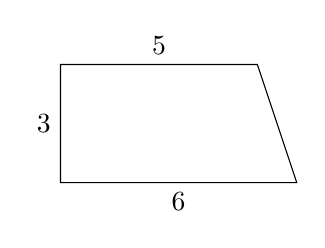
\begin{tikzpicture}[scale=0.5]
\draw (0,0) -- (0,3) -- (5,3) -- (6,0) -- cycle;
\path (0,0) -- (0,3) node [left, midway] {3};
\path (0,3) -- (5,3) node [above, midway] {5};
\path (0,0) -- (6,0) node [below, midway] {6};
\end{tikzpicture}
\end{multicols}
\item Which is warmer, 48\degree\C or 112\degree\F?
\item Which is colder, 18\degree\C or 53 \degree\F?
\item What is the melting point of gold in \degree\F if its melting point is 1,115 \degree\C?
\item What is the melting point of silver in \degree\C if its melting point is 1,814 \degree\F?
\end{enumerate}

\subsection*{Activity 2: Math Trail}
\subsection*{Objective:}
To apply measurement skills, conversion, and problem solving in real-life situations.
\subsection*{Preparation:}
Group the participants into groups. Each group is oriented on the rules of the “Math Trail”/Amazing Race”.
\subsection*{Instructions:}
Using the same materials (e.g. ruler, meterstick, protractor, calculator), each group will race
in a specified area (an auditorium or field) to do tasks (e.g. measure, compute) in a given
time limit.
\subsection*{Sample Task 1:}
Assume that the figures drawn are a square and a circle.
Find the area of the shaded region rounded to the nearest $\mm^2$.
\begin{figure}[!h]
\centering
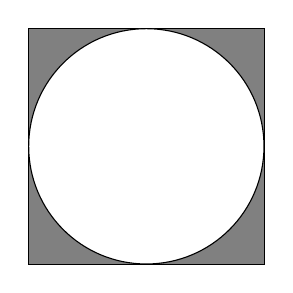
\begin{tikzpicture}[scale=1.5]
\draw [fill=gray] (-1,-1) -- (1,-1) -- (1,1) -- (-1,1) -- cycle;
\node (a) [circle, text width=3cm, inner sep=0pt,draw,fill=white] {};
\end{tikzpicture}
\end{figure}

\subsection*{Sample Task 2:}

Assume that the figures drawn are a triangle and a circle.

Find the volume of the cylinder whose base radius is the same as
the circumference of the circle and whose height is the same as the
perimeter of the triangle (rounded to the nearest $\mL$).\\

\begin{figure}[!h]
\centering
\begin{tikzpicture}[scale=2.5]
\coordinate (a) at ($(0,0)+(90:0.5cm)$);
\coordinate (b) at ($(0,0)+(-30:0.5cm)$);
\coordinate (c) at ($(0,0)+(-150:0.5cm)$);
\draw [fill=gray,opacity=0.5] (a) -- (b) -- (c) -- cycle;
\draw (0,0) circle (0.5cm);
\end{tikzpicture}
\end{figure}
